% Configuración de la clase (Español, PDF y tamaño 11pt)
\documentclass[spanish]{pucthesis}

%%%%%%%%%%%%%%%%%%%%%%%%%%%%%
%%   Paquetes esenciales   %%
%%%%%%%%%%%%%%%%%%%%%%%%%%%%%

% Gráficos y figuras
\usepackage{graphicx}
\usepackage{float}
\usepackage{subcaption}
\usepackage{xcolor}

% Paquetes matemáticos
\usepackage{amsfonts}
\usepackage{amssymb}

% Tipografía
\usepackage{enumitem}

% Diseño de tablas
\usepackage{booktabs}
\usepackage{multirow}
\usepackage{array}
\captionsetup[table]{
    singlelinecheck=false,
    justification=raggedright,
    labelsep=newline,
    labelfont=bf,
    textfont=it
}
\usepackage{pgfgantt}

% Ajuste para evitar errores de espaciado en la bibliografía
\usepackage{etoolbox}
\apptocmd{\sloppy}{\hbadness 10000\relax}{}{}

\makeatletter
\patchcmd{\chapter}{\if@openright\cleardoublepage\else\clearpage\fi}{\par}{}{}
\patchcmd{\chapter}{\clearpage}{\par}{}{}
\makeatother

\renewcommand{\cleardoublepage}{\par}
\renewcommand{\clearpage}{\par}

% Citas, referencias (Formato APA tradicional con apacite) y enlaces en el PDF
\usepackage[hidelinks,pdfusetitle,pdfdisplaydoctitle]{hyperref}
\usepackage[notocbib]{apacite} 
\usepackage{doi}
\renewcommand{\doitext}{}

%--------------------------------------%
% Entornos matemáticos y de definición %
%--------------------------------------% 
\newtheorem{definition}{\bf Definición}[chapter]
\newtheorem{property}{Propiedad}[chapter]
\newtheorem{lemma}{\bf Lema}[chapter]
\newtheorem{proposition}{Proposición}[chapter]
\newtheorem{theorem}{\noindent \bf Teorema}[chapter]
\newtheorem{corollary}{\bf Corolario}[chapter]
\newtheorem{pf}{Demostración}[chapter]
\newtheorem{example}{\bf Ejemplo}[chapter]
\newtheorem{remark}{Observación}[chapter]

% Ajuste de espacio para evitar que la portada se pase a otra página
\makeatletter
  \setlength{\beftitle}{60\p@\@plus24\p@} % Se reduce el espacio antes del título
  \setlength{\afttitle}{40\p@}            % Se reduce el espacio después del título
\makeatother

\raggedbottom

%%%%%%%%%%%%%%%%%%%%%%%%%%%%%
%%%%%%%   Documento   %%%%%%%
%%%%%%%%%%%%%%%%%%%%%%%%%%%%%

\begin{document}

\title[Postergación del Etiquetado en una Viña Exportadora bajo Incertidumbre en la Demanda \\ GRUPO 8]{\bf Postergación del Etiquetado en una Viña Exportadora bajo Incertidumbre en la Demanda \\ GRUPO 8}

\author[Integrantes:]{Integrantes:\\
\textnormal{\small{
Javiera Isidora Andrade Rodríguez\\
Pía Francisca Ayala Nanjari\\
Rafael Alfonso Calderón Avendaño\\
Valentina Andrea Gallegos Bravo\\
Francisco Ignacio Indo Maza\\
Aline Kneuer van Baal}
}
}

\address{Escuela de Ingeniería\\
         Pontificia Universidad Católica de Chile\\
         Vicuña Mackenna 4860\\
         Santiago, Chile}

\advisor{\textbf{Profesor Guía:} Sergio Maturana}
\ogrsmember{\textbf{Ayudante Tutor:} Ignacio Peña}
\date{Septiembre 2026}
\copyrightname{Grupo 8}
\copyrightyear{2026}

%%%%%%%%%%%%%%%%%%%%%%%%%%%%%%
%%  Portada y preliminares  %%
%%%%%%%%%%%%%%%%%%%%%%%%%%%%%%

\NoChapterPageNumber
\pagenumbering{roman}
\maketitle

%%%%%%%%%%%%%%%%%%%%%%%%%%%%%%%
%%%%%%%%    Índices    %%%%%%%%
%%%%%%%%%%%%%%%%%%%%%%%%%%%%%%%

\pdfbookmark{\contentsname}{toc}
\newpage
\tableofcontents
\phantomsection \label{lista_figuras}
\listoffigures
\phantomsection \label{lista_tablas}
\listoftables
\cleardoublepage

%------------------------------------%

%%%%%%%%%%%%%%%%%%%%%%%%%%%%%%%
%%%%%%%%    Resumen    %%%%%%%%
%%%%%%%%%%%%%%%%%%%%%%%%%%%%%%%

\phantomsection \label{resumen}
\chapter*{RESUMEN}
Las viñas orientadas a la exportación enfrentan un problema de planificación del envasado en el que cada producto terminado corresponde a una combinación única de vino y etiqueta, determinada por el idioma, la normativa sanitaria y los requerimientos comerciales de cada mercado de destino. Dado que los pronósticos de los importadores son poco precisos, comprometer anticipadamente el etiquetado expone a la viña a mantener inventario en combinaciones que la demanda no valida, mientras que producir exclusivamente contra pedido multiplica los tiempos de preparación y presiona la capacidad de la línea. La postergación del etiquetado, consistente en almacenar botellas llenas sin etiquetar hasta disponer de información de demanda más precisa, constituye un punto intermedio cuyo valor económico es necesario cuantificar.

Este informe corresponde a la primera etapa del proyecto, orientada a caracterizar el problema y a definir la estrategia de modelación. Se realizó un análisis exploratorio de la instancia base, correspondiente a una viña con dos vinos, cinco combinaciones vino--etiqueta y una demanda representada mediante un árbol de escenarios de tres períodos y once nodos. El análisis verificó la consistencia probabilística del árbol, caracterizó la demanda esperada y su variabilidad por producto, y estimó la estructura de correlación entre productos. Los resultados muestran correlaciones heterogéneas entre etiquetas que comparten un mismo vino base, condición bajo la cual la literatura reporta los mayores beneficios de la postergación, y sugieren que la capacidad de la línea no constituiría la restricción activa del problema.

Sobre esa base se selecciona la optimización estocástica multietapa como metodología y se formula un modelo preliminar de embotellado y etiquetado, junto con los indicadores de desempeño y el diseño experimental que permitirán cuantificar el valor de la postergación en las etapas siguientes.

\vfill
\noindent {\bf Palabras Claves}: postergación del etiquetado, optimización estocástica multietapa, planificación del envasado, incertidumbre en la demanda, industria vitivinícola.

%%%%%%%%%%%%%%%%%%%%%%%%%%%%%%%%
%%%%%  Cuerpo del Informe  %%%%%
%%%%%%%%%%%%%%%%%%%%%%%%%%%%%%%%

\pagenumbering{arabic}

\newpage

\chapter{Introducción}
El mercado internacional del vino es un entorno altamente competitivo y fragmentado. Globalmente, se producen más de 28 mil millones de litros de vino anuales repartidos en 57 países productores, sin que ninguno supere el 17\% de la participación de mercado \cite{varas2018}. En este contexto, la industria vitivinícola chilena está fuertemente orientada a la exportación, atendiendo clientes en múltiples canales de venta extranjeros \cite{varas2018}.

\section{Contexto del Negocio y Estructura del Canal\label{sec:sub1}}
Las viñas chilenas orientadas a la exportación comercializan su producción principalmente a través de grandes intermediarios, importadores internacionales o grandes cadenas de distribución minorista, más que mediante una venta directa al consumidor final \cite{bouzdine2011}. Esta dinámica concentra la negociación comercial en un grupo reducido de clientes de gran volumen. Dicha estructura se alinea con lo reportado en la literatura sobre la cadena de suministro vitivinícola nacional, la cual caracteriza a la industria exportadora por una marcada disparidad estructural entre un grupo minoritario de viñas de gran escala que concentra la mayor parte del volumen exportado, y una base atomizada de pequeños productores de uva \cite{reinecke2023}.

Esta concentración comercial simplifica las transacciones globales, pero introduce una alta complejidad a nivel operacional y de planta: cada cliente demanda habitualmente lotes en formatos estandarizados (por ejemplo, cajas de 6 o 12 botellas de 750 ml), pero bajo requerimientos estrictamente diferenciados de marca, línea comercial (económica, media o premium) y, de manera crítica para este proyecto, etiquetas específicas, a pesar de que el vino contenido en el envase sea exactamente el mismo \cite{cholette2018, varas2018}. Como consecuencia, los productos destinados a diferentes mercados geográficos no pueden ser tratados como sustitutos comerciales, a pesar de contener exactamente el mismo vino líquido \cite{cholette2009}.

\section{El Etiquetado como Problema Central\label{sec:sub2}}
Aunque el vino embotellado sea físicamente idéntico, la etiqueta debe adaptarse de manera única por al menos cuatro motivos fundamentales:

\begin{enumerate}
    \item \textbf{Idioma:} Cada mercado de destino exige su propio idioma en la etiqueta, limitando la intercambiabilidad del inventario entre mercados idiomáticos distintos \cite{bouzdine2011}.
    \item \textbf{Normativa Sanitaria y Legal:} Cada país exige advertencias distintas sobre el consumo de alcohol y menciones obligatorias de origen. En Chile, la Ley N.° 18.455 \cite{minagri1985} y su respectivo reglamento, el Decreto N.° 78 de 1986 del Ministerio de Agricultura \cite{minagri1986}, ambos fiscalizados por el Servicio Agrícola y Ganadero (SAG), exigen que los envases o etiquetas indiquen, como mínimo, la denominación, graduación alcohólica (con un mínimo de 11,5° para consumo directo), volumen y país de origen (incorporando la mención obligatoria ``Envasado en Chile'' o ``Embotellado en Chile'' para partidas de exportación) \cite{minagri1985}. Aunque el contenido conceptual sea similar entre países vecinos (por ejemplo, Chile y Argentina), la redacción legal requerida cambia, obligando a usar etiquetas físicamente diferenciadas.
    \item \textbf{Motivos Comerciales:} Los grandes compradores internacionales exigen frecuentemente el uso de marcas blancas o exclusivas, requiriendo un diseño de etiqueta diferenciado para su canal de comercialización \cite{bouzdine2011}.
    \item \textbf{Diseño de Etiqueta y Estrategia de Posicionamiento:} Las viñas adaptan los elementos estéticos (colores, tipografía y códigos visuales) a las preferencias culturales de cada mercado de destino con el fin de posicionar un mismo vino en segmentos comerciales variados (por ejemplo, estilos clásicos para mercados tradicionales versus diseños minimalistas para mercados contemporáneos) \cite{cholette2009}.
\end{enumerate}
El principal problema radica en que los pronósticos de pedidos de importación son altamente inexactos debido a la estacionalidad del negocio, los tiempos de transporte prolongados y las variaciones en las preferencias de los consumidores \cite{cholette2009, varas2018}. Planificar bajo un enfoque tradicional de fabricación para inventario (\textit{Make-to-Stock} o MTS) genera un alto riesgo de asignación errónea de producto (\textit{product misallocation}), lo que provoca simultáneamente costosas rupturas de \textit{stock} en algunos canales y excesos de inventario obsoleto en otros \cite{cholette2009, varas2018}.

\section{Comparación de Esquemas de Planificación Extremos\label{sec:sub3}}
Frente a esta multiplicidad de combinaciones vino--etiqueta, la viña puede optar por dos esquemas extremos de planificación:

\begin{itemize}
    \item \textbf{Producir contra stock (MTS)}: Fabricar y almacenar producto terminado listo para el despacho inmediato. Sin embargo, para una viña exportadora es inviable mantener \textit{stock} terminado de todas las combinaciones posibles de vino, etiqueta y mercado debido a la imprevisibilidad de los importadores y al riesgo de obsolescencia \cite{cholette2009}. Además, cambiar la etiqueta de una botella ya envasada es una operación cara y lenta, ya que implica lavar, secar y manipular botellas que ya están llenas de líquido, exponiéndolas a riesgos de rotura o mermas de calidad \cite{cholette2018}.

    \item \textbf{Producir contra pedido (MTO)}: Fabricar exclusivamente tras recibir la orden del cliente. Aunque elimina el inventario obsoleto, castiga severamente los tiempos de respuesta y satura las líneas de embotellado debido a los tiempos de preparación dependientes de la secuencia (\textit{sequence-dependent set-up times}), donde alternar la producción entre distintas familias de vinos incrementa los tiempos de lavado y merma drásticamente la capacidad de planta \cite{maccawley2022}.
\end{itemize}

\section{Planteamiento de la Oportunidad\label{sec:sub4}}
Si la viña logra desacoplar correctamente el embotellado del etiquetado, establece un punto de desacople (\textit{decoupling point}) estratégico en el inventario intermedio de botellas llenas sin etiquetar (\textit{Work-In-Process} o WIP). Este punto divide el flujo logístico en dos fases: una fase de embotellado empujada (\textit{push}) basada en pronósticos agregados de vino base, y una fase de etiquetado tirada (\textit{pull}) gatillada por los pedidos en firme de los clientes internacionales \cite{cholette2009, varas2018}. Este desacople permite reducir drásticamente el inventario terminado que hoy se mantiene ``atrapado'' en combinaciones rígidas de vino--etiqueta que no siempre calzan con la demanda real, liberando de esta manera capital de trabajo y capacidad de almacenamiento físico en la bodega \cite{cholette2009, varas2018}.

No obstante, la implementación de esta práctica introduce complejidades operacionales no menores: las líneas de producción disponen de una capacidad limitada de horas por período y se alimentan desde un número acotado de estanques intermedios, lo que limita la cantidad de variedades de vino base que pueden ser procesadas simultáneamente y obliga a secuenciar meticulosamente los ciclos para mitigar los costosos \textit{set-ups} mayores y menores \cite{maccawley2022}.

A pesar de estas restricciones, la postergación otorga una valiosa flexibilidad comercial. La bodega puede aceptar pedidos urgentes de nuevos clientes o absorber cancelaciones y modificaciones de última hora sin necesidad de reprogramar la línea de embotellado desde cero, puesto que el vino ya se encuentra envasado de forma genérica (\textit{``blanks''}) y solo resta aplicarle la etiqueta específica de destino \cite{cholette2009, varas2018}. En un contexto global donde las exigencias regulatorias y comerciales de cada mercado de destino cambian constantemente, esta flexibilidad es un factor de competitividad clave frente a viñas competidoras que producen de forma rígida contra \textit{stock} terminado y diferenciado.

Para abordar este desafío, el proyecto diseña una metodología de apoyo a la toma de decisiones basada en Investigación Operativa que permite evaluar los beneficios de postergar el etiquetado en una viña exportadora bajo incertidumbre en la demanda. La motivación, el objetivo general y los entregables comprometidos se formalizan en la Sección~\ref{sec:sec6}. \\

\vspace{0.5cm}

\chapter{Descripción detallada del problema} \label{sec2}
La etapa de empaque vitivinícola posee características particulares que configuran un problema de programación altamente complejo (\textit{Np-Hard}) \cite{maccawley2022, varas2018}.

\section{El Proceso de Embotellado y Tipos de \textit{Set-ups}\label{sec:sec1}}
Las bodegas de gran escala operan múltiples líneas de producción en paralelo, las cuales se abastecen desde tanques de almacenamiento intermedio \cite{varas2018}.
Cuando ambas operaciones se realizan de manera acoplada, la
velocidad general de la línea queda determinada por el etiquetado, que suele ser más lento que el embotellado \cite{varas2018}. Los cambios de producción generan dos tipos de \textit{set-ups}. Los \textit{set-ups} mayores ocurren al modificar la familia de botellas, por ejemplo, su tamaño, forma o color \cite{bouzdine2011}, y requieren desmontar y calibrar componentes de la línea, pudiendo detenerla durante un turno completo de ocho horas. \cite{maccawley2022}. 

Los \textit{set-ups} menores corresponden a cambios de SKU, etiqueta o variedad de vino dentro de una misma familia de botellas y requieren entre 20 y 60 minutos \cite{maccawley2022}. Estos tiempos también dependen de la secuencia de producción. Por ello, una secuencia inadecuada puede destinar entre un 15\% y un 40\% del tiempo productivo a detenciones por \textit{set-ups}, haciendo que la secuenciación sea una decisión relevante para el uso de la capacidad \cite{maccawley2022}.

\section{La Postergación del Etiquetado (\textit{Labelling Postponement}) como Estrategia de Cobertura\label{sec:sec3}}

La postergación consiste en retener las botellas llenas de vino en un estado intermedio sin etiquetar (\textit{“blancks”}) en el almacén, retrasando el proceso de etiquetado final hasta recibir información de demanda más precisa de los importadores \cite{cholette2009, varas2018}.

\subsection{Desventaja (Costo de \textit{Postponement}): \label{sec:sub1_desv}}
Romper el flujo continuo e introducir un doble manejo de botellas aumenta los costos de preparación, ya que se incurre en un \textit{set-up} de embotellado y posteriormente en un \textit{set-up} de etiquetado independiente, en lugar de uno conjunto). Además, genera costos adicionales de almacenamiento físico para el inventario intermedio \cite{cholette2009, varas2018}.

\subsection{Ventaja\label{sec:sub2_vent}}
Proporciona una flexibilidad operativa sustancial. \cite{varas2018} demostraron que la postergación ofrece mayores beneficios económicos bajo tres condiciones específicas: $1^{ro}$, cuando la capacidad de producción es moderadamente ajustada. Si es extremadamente holgada o saturada, el beneficio marginal de la flexibilidad decrece significativamente; $2^{do}$, cuando la variabilidad de la demanda es alta en los mercados de exportación, y $3^{ro}$, cuando existe una correlación negativa en la demanda entre los diferentes SKUs, permitiendo compensar las alzas de un mercado con las bajas de otro utilizando el mismo \textit{stock} de botellas sin etiquetar.

\section{Restricciones Regulatorias y de Etiquetado\label{sec:sec4}}


El etiquetado de vinos está rígidamente normado por leyes nacionales e internacionales, lo que incrementa la fragmentación de inventario y la necesidad de postergación:

\begin{itemize}
    \item En Chile, la Ley 18.455 (Decreto N.° 78 de 1986) exige que la etiqueta indique denominación, graduación alcohólica, volumen, envasador y la mención "Envasado/Embotellado en Chile" para exportación.
    
    \item En la Unión Europea, el Reglamento (UE) 2021/2117 exige incorporar información nutricional e ingredientes en el etiquetado. Estas exigencias, distintas por país aunque el vino base sea el mismo, aceleran la obsolescencia de etiquetas ya impresas y refuerzan la necesidad de postergar la diferenciación \cite{bouzdine2011,varas2018}.

\end{itemize}

\section{Motivación, Objetivo General y Entregables del Proyecto\label{sec:sec6}}

\begin{enumerate} [label = \arabic*.]
    \item \textbf{Motivación:} Surge de la ineficiencia crónica y el riesgo financiero asociados al esquema tradicional MTS/MTO en la bodega (Cholette, 2009). La alta inexactitud de los pronósticos de importación genera el riesgo de asignación errónea de producto, lo que provoca costosas rupturas de stock y excesos de inventario obsoleto, agravado por las normativas de etiquetado nacional (Ley 18.455) e internacional (Reglamento UE 2021/2117) que fragmentan el stock e impiden su libre intercambio (Bouzdine-Chameeva \& Cholette, 2011; Varas et al., 2018).

    \item \textbf{Objetivo General:} Diseñar una metodología cuantitativa de apoyo a la toma de decisiones basada en Investigación Operativa que permita evaluar los beneficios de implementar la postergación táctica del etiquetado en una viña exportadora bajo incertidumbre en la demanda, determinando de manera óptima los lotes a embotellar y etiquetar en cada período en tiempos de cómputo razonables.
    
    \item \textbf{Entregables:} Se entregará un modelo de optimización implementado computacionalmente, junto con un análisis de resultados que permita comparar distintas políticas de producción y cuantificar el valor económico de postergar el etiquetado bajo diferentes escenarios de demanda, capacidad y variabilidad.

    \end{enumerate}

\section{Análisis Exploratorio de los Datos de la Instancia Base\label{sec:s0}}

Se realizó un análisis exploratorio de la instancia de datos entregada por el profesor (Anexo A), correspondiente a una viña que produce dos vinos, Vino 1 y Vino 2, sobre una única línea de envasado capaz de embotellar y etiquetar de forma acoplada o desacoplada. El Vino 1 admite tres etiquetas y el Vino 2 admite dos, lo que da origen a cinco combinaciones vino-etiqueta cuya demanda se conoce a través de un árbol de escenarios de tres períodos y once nodos, calibrado con estados de demanda alta, media y baja.


\section{Decisiones, objetivos, restricciones e indicadores de desempeño}

\label{subsec:decisiones_objetivos_restricciones}
La planificación del envasado enfrenta un \textit{trade-off} entre diferenciar anticipadamente el producto y conservar flexibilidad frente a la incertidumbre de la demanda. Retrasar el etiquetado permite mantener inventario genérico hasta disponer de mayor información, reduciendo el riesgo de asignar producto a una
etiqueta cuya demanda futura resulte menor a la prevista
\citep{cholette2009,varas2018}.

Esta flexibilidad, sin embargo, implica costos adicionales de inventario, \textit{set-ups} y capacidad. Por ello, la decisión consiste en determinar si el beneficio de conservar capacidad de reasignación compensa dichos costos operacionales.

\subsection{Estructura de decisión bajo incertidumbre}

La demanda se representa mediante un árbol de escenarios de tres períodos y once nodos, donde cada nodo resume la información disponible hasta ese momento. Las decisiones pueden adaptarse a la demanda observada, pero no utilizar información futura, respetando el principio de no anticipatividad. Además, lo embotellado en un período queda disponible una etapa después. Por ello, el embotellado constituye una decisión \textit{ex ante}, mientras que el etiquetado de inventario previamente embotellado funciona como una decisión de recurso, al poder ajustarse una vez revelada nueva información. Esta secuencia permite desplazar parte de la diferenciación hacia un momento de menor incertidumbre, constituyendo el principal mecanismo mediante el cual la postergación puede generar valor económico.

\subsection{Decisiones principales}

Se identifican tres decisiones operacionales principales:

\begin{itemize}
    \item \textbf{Embotellado sin etiquetar:} definir cuánto vino embotellar y mantener como inventario genérico, conservando flexibilidad entre las etiquetas compatibles.

    \item \textbf{Embotellado y etiquetado acoplados:} definir cuánto producir directamente como una combinación vino--etiqueta, evitando una operación posterior pero comprometiendo anticipadamente el inventario.

    \item \textbf{Etiquetado de inventario intermedio:} asignar las botellas genéricas disponibles a productos finales compatibles según la información de demanda revelada, materializando la estrategia de postergación.
\end{itemize}

Estas decisiones se complementan con la activación de \textit{set-ups}, la gestión de inventarios y el tratamiento de pedidos atrasados.

\subsection{Objetivo operacional}

El objetivo operacional es determinar una política de embotellado, etiquetado e inventario que minimice el costo total esperado a lo largo del árbol de escenarios. Para ello, los costos de cada nodo se ponderan por su probabilidad de ocurrencia, incorporando explícitamente las distintas realizaciones posibles de la demanda.
Para una configuración experimental dada, la función objetivo se expresa conceptualmente como:

\begin{equation}
\min \;
\sum_{n\in\mathcal{N}} p_n
\left[
    C^{setup}_n
    +C^{WIP}_n
    +C^{FG}_n
    +C^{BO}_n
\right],
\label{eq:objetivo_esperado}
\end{equation}

donde $C^{setup}_n$ incorpora los \textit{set-ups} de embotellado,
embotellado-etiquetado y etiquetado; $C^{WIP}_n$ corresponde al inventario de
botellas sin etiquetar; $C^{FG}_n$ al inventario de producto terminado; y
$C^{BO}_n$ a los pedidos atrasados. Su formulación algebraica con los
parámetros de la instancia se presenta en el Anexo~\ref{anexo:restricciones}. La estructura de costos penaliza fuertemente los pedidos atrasados: una
botella--período de atraso equivale al costo de almacenar 1.000 botellas terminadas o 1.500 botellas sin etiquetar durante un período. Así, aunque el modelo minimiza un único costo total esperado, la parametrización prioriza implícitamente el cumplimiento oportuno de la demanda. Sin embargo, el valor óptimo no caracteriza por sí solo el desempeño de una política, por lo que las soluciones se complementarán con los indicadores definidos en la sección siguiente.

\section{Objetivos de evaluación e indicadores de desempeño}

Los indicadores de desempeño permiten evaluar las políticas desde cuatro dimensiones complementarias: eficiencia económica, cumplimiento de la demanda, valor de la postergación y beneficio de la adaptación multietapa. A partir de estas dimensiones se definen los siguientes objetivos de evaluación:

\begin{enumerate}[label=\textbf{KPI-\arabic*.}, leftmargin=*, itemsep=2pt]
    \item Evaluar la eficiencia económica global de las políticas obtenidas y permitir su comparación bajo una misma configuración experimental.
    \item Evaluar la capacidad de la política para satisfacer la demanda dentro del período en que es requerida.
    \item Cuantificar el beneficio económico atribuible específicamente a disponer de diferenciación tardía.
    \item Cuantificar el beneficio atribuible a adaptar las decisiones a medida que se revela nueva información, distinguiéndolo del beneficio físico de mantener producto sin diferenciar.
    \item Determinar si ampliar el nivel de postergación genera rendimientos decrecientes e identificar qué productos concentran primero su valor.
\end{enumerate}

\medskip
\noindent\textbf{KPI-1. Costo total esperado: }El costo total esperado corresponde a la medida de \textbf{eficiencia económica} de la política y coincide con el criterio de optimización utilizado por el modelo. Se calcula como
\begin{equation}
    CTE =
    \sum_{n\in\mathcal{N}}p_n
    \left(
        C^{setup}_n+
        C^{WIP}_n+
        C^{FG}_n+
        C^{BO}_n
    \right),
\end{equation}

donde $p_n$ es la probabilidad de alcanzar el nodo $n$. Se expresa en \textbf{unidades monetarias} y, entre políticas evaluadas bajo una misma configuración, un menor $CTE$ indica un mejor desempeño económico esperado.

\medskip
\noindent\textbf{KPI-2. Nivel de servicio: }El nivel de servicio representa el \textbf{desempeño en el cumplimiento temporal de la demanda}. Se define como la proporción esperada de unidades cuya demanda es satisfecha dentro del período en que son requeridas:
\begin{equation}
    NS =
    \frac{
        \mathbb{E}[\text{demanda satisfecha oportunamente}]
    }{
        \mathbb{E}[\text{demanda total}]
    }
    \times100\%.
\end{equation}

Es adimensional y se expresa como porcentaje: un valor de $100\%$ implica ausencia de pedidos atrasados, y valores inferiores, demanda desplazada a períodos posteriores.

\medskip
\noindent\textbf{KPI-3. Valor económico de la postergación: }El valor económico de la postergación mide la reducción del costo total esperado atribuible a la diferenciación tardía. Para una configuración experimental $\theta$, que fija las condiciones de capacidad, variabilidad y correlación de la demanda, y un nivel de postergación $PL>0$, se define como:
\begin{equation}
    V^{POST}(PL;\theta)
    =
    CTE^{*}(0;\theta)
    -
    CTE^{*}(PL;\theta).
\end{equation}

Se expresa en las mismas \textbf{unidades monetarias} del costo total esperado. Un valor positivo indica, \textit{ceteris paribus}, que permitir postergación reduce el costo esperado; uno negativo, que los costos adicionales de la estrategia superan el beneficio de la mayor flexibilidad.

\medskip
\noindent\textbf{KPI-4. Valor de la solución multietapa (VMS): }El VMS cuantifica el beneficio de la adaptación temporal de las decisiones frente a la revelación progresiva de incertidumbre, comparando el costo óptimo de una formulación con menor capacidad adaptativa con el del modelo multietapa:

\begin{equation}
    VMS =
    Z^{*}_{2\text{-etapas}}
    -
    Z^{*}_{\text{multietapa}}.
\end{equation}

Un valor positivo indica que la adaptación secuencial de las decisiones reduce el costo esperado. Así, el VMS captura el valor informacional y temporal de la adaptación, diferenciándolo del valor económico de la postergación, asociado a mantener producto sin diferenciar.

\medskip
\noindent\textbf{KPI-5. Valor marginal de ampliar la flexibilidad: }Cuantifica la reducción adicional del costo óptimo esperado obtenida al aumentar el nivel de postergación entre dos configuraciones consecutivas. Para dos niveles $PL_a < PL_b$, se define como
\begin{equation}
    \Delta V_{a,b} = Z^*_{PL_a} - Z^*_{PL_b}.
    \label{eq:valor_marginal}
\end{equation}

La comparación sucesiva entre niveles de $PL$ permite detectar la existencia de rendimientos decrecientes de la postergación e identificar qué productos prioriza el modelo al ampliar progresivamente la posibilidad de diferenciación tardía.


\subsection{Restricciones principales}

Las restricciones representan las condiciones físicas, temporales y operacionales
que delimitan las políticas factibles. En esta sección se presentan
conceptualmente, mientras que su formulación algebraica se incluye en el
Anexo~\ref{anexo:restricciones}.

\medskip
\noindent\textbf{Conservación del inventario intermedio: } El inventario de botellas sin etiquetar en cada período corresponde al inventario remanente y al embotellado previamente disponible, descontando las unidades destinadas a etiquetado. Esta restricción asegura la conservación física del producto e impide utilizar unidades antes de que estén disponibles. La restricción se presenta en el Anexo \nameref{eq:anexoD-balance-intermedio}.

\medskip
\noindent\textbf{Conservación de producto terminado y demanda pendiente: }Para cada combinación vino--etiqueta, la demanda debe ser satisfecha mediante producto terminado disponible o mediante producto que pueda completarse en el período correspondiente. La demanda no satisfecha se conserva como pedido atrasado. Esta permite representar explícitamente el vínculo entre producción, inventario y cumplimiento de los requerimientos de demanda. Veáse Anexo \nameref{eq:anexoD-balance-terminado}.

\medskip
\noindent\textbf{Capacidad de la línea: }Las operaciones de embotellado, etiquetado, producción acoplada y sus respectivos \textit{set-ups} comparten la misma capacidad productiva. Dado que la postergación utiliza la línea tanto en el embotellado como en el etiquetado posterior, su beneficio debe compensar este uso adicional de capacidad
\citep{maccawley2022}. 
Véase Anexo Anexo \nameref{eq:anexoD-capacidad}.

\medskip
\noindent\textbf{Activación de \textit{set-ups}: }Toda operación productiva requiere activar su preparación correspondiente,
incorporando su tiempo y costo fijo. Esto evita fragmentar artificialmente la
producción sin considerar sus consecuencias operacionales. Las restricciones
se presentan en el Anexo \nameref{eq:anexoD-setup-embotellado}.

\medskip
\noindent\textbf{Compatibilidad vino--etiqueta: }El inventario sin etiquetar solo puede reasignarse entre etiquetas compatibles
con el mismo vino base. Así, el \textit{risk pooling} generado por la
postergación ocurre dentro de cada familia de productos y no permite sustituir
inventario entre vinos distintos \citep{cholette2009,varas2018}. Véase Anexo \nameref{eq:anexoD-compatibilidad}.

\medskip
\noindent\textbf{Disponibilidad de estanques:}Los 20 estanques de 10.000 litros limitan el volumen de vino preparado
simultáneamente antes del embotellado. Estos no corresponden a almacenamiento
de botellas sin etiquetar y, por tanto, se distinguen del inventario intermedio
generado por la postergación. Véase Anexo \nameref{eq:anexoD-numero-estanques}.

\medskip
\noindent\textbf{Condiciones iniciales y de frontera temporal: }La formulación debe respetar los inventarios y pedidos atrasados iniciales, así
como el horizonte finito de planificación. En particular, las decisiones del
último período no deben generar beneficios asociados a producto disponible
fuera del horizonte, salvo que se defina explícitamente un valor residual.

 
\subsection{Metodología\label{sec:s1}}

El análisis se implementó en Python, de forma reproducible y fácil de actualizar ante cambios en los datos base, y comprende cuatro etapas: (i) validar la consistencia probabilística del árbol de escenarios, (ii) calcular estadística descriptiva y demanda esperada por producto, (iii) estimar la correlación de demanda entre las cinco combinaciones vino--etiqueta, y (iv) evaluar, nodo a nodo, las horas de línea requeridas frente a la capacidad disponible bajo el supuesto extremo de que todo el volumen se embotella y etiqueta de forma acoplada, es decir, sin aprovechar la postergación. Este último supuesto se adoptó como cota superior del uso de capacidad, ya que interesa comprobar si esta puede llegar a ser una restricción activa incluso en el escenario que menos se beneficia de desacoplar el etiquetado.

\subsection{Consistencia del Árbol de Escenarios\label{sec:s2}}

La validación confirmó la consistencia probabilística del árbol: las
probabilidades condicionales de los nodos hijos suman uno y las probabilidades de los escenarios terminales también totalizan uno. La estructura completa se presenta en la Figura~\ref{fig:anexo_arbol} del
Anexo~\ref{anexo:graficos}. Por ello, los datos pueden utilizarse directamente como parámetros del modelo estocástico, sin ajustes adicionales.




\subsection{Caracterización de la Demanda por Producto\label{sec:s3}}

La demanda esperada, ponderada por la probabilidad de cada nodo terminal,
resultó heterogénea entre los cinco productos, como se presenta en la
Figura~\ref{fig:anexo_demanda_esperada} del
Anexo~\ref{anexo:graficos}. La combinación $(1,1)$ concentra la mayor demanda
esperada (40.665 botellas), pero también la mayor variabilidad relativa
(coeficiente de variación de $0{,}59$, con un máximo de 81.856 botellas frente
a un mínimo de 10.426 según el nodo), mientras que las combinaciones del
Vino 2, $(2,1)$ y $(2,2)$, presentan una demanda esperada más moderada
(26.732 y 25.165 botellas, respectivamente) y sensiblemente más estable
(coeficiente de variación cercano a $0{,}33$). La combinación $(1,3)$ es la
de menor demanda esperada (16.901 botellas). Esta heterogeneidad sugiere que
el valor de postergar el etiquetado no debiese ser uniforme entre vinos, sino
que dependerá de cuán variable es la demanda de cada combinación
vino--etiqueta.



\subsection{Estructura de Correlación y Valor de la Postergación\label{sec:s4}}

Un resultado especialmente relevante para el problema en estudio es la
estructura de correlación de la demanda entre productos, cuya matriz completa
se presenta en la Figura~\ref{fig:fig3} del Anexo~\ref{anexo:graficos}.
Las etiquetas del Vino 1 presentan correlaciones negativas en dos de sus
combinaciones (por ejemplo, $-0{,}66$ entre las combinaciones $(1,1)$ y
$(1,2)$), mientras que las dos etiquetas del Vino 2 se correlacionan de forma
casi perfecta y positiva ($0{,}98$ entre $(2,1)$ y $(2,2)$).

Este hallazgo respalda la lógica de la postergación como punto de desacople: cuando las demandas de etiquetas asociadas a un mismo vino se mueven en direcciones opuestas, el inventario sin etiquetar puede reasignarse hacia el producto con mayor demanda, reduciendo la necesidad de mantener inventarios diferenciados por adelantado \cite{cholette2018}. Por ello, el efecto de \textit{risk pooling} resulta más prometedor para el Vino 1, donde predominan correlaciones negativas entre etiquetas, que para el Vino 2, cuyas demandas presentan una correlación fuertemente positiva y, por tanto, menor capacidad de compensación.


Se estimaron las horas de línea requeridas en los once nodos bajo producción acoplada y sin postergación. En ningún caso se superan las 84 horas disponibles por período, observándose una holgura mínima de 29,5 horas en el nodo de mayor demanda del período 2. Este resultado sugiere que, bajo esta estimación simplificada, la capacidad no sería la principal restricción de la instancia base. Sin embargo, los
\textit{set-ups} dependientes de la secuencia y la interacción entre
embotellado, etiquetado e inventarios podrían aumentar su utilización efectiva \cite{maccawley2022}. Por ello, se espera que el valor de la postergación se manifieste principalmente en una mejor asignación del inventario y en la reducción de pedidos atrasados, cuya penalización alcanza \$15.000 por botella y período, más que en la factibilidad básica de satisfacer la demanda.
\subsection{Conclusiones del Análisis Exploratorio\label{sec:s6}}

El análisis exploratorio entrega tres conclusiones principales para orientar la modelación. Primero, los datos y la estructura probabilística del árbol son consistentes, por lo que pueden utilizarse directamente como parámetros del
modelo estocástico. Segundo, las diferencias en la correlación de la demanda sugieren que el valor de la postergación no será homogéneo entre productos: el Vino 1, con correlaciones predominantemente negativas entre sus etiquetas, presenta mayor potencial de \textit{risk pooling} que el Vino 2. Tercero, la holgura observada en el análisis preliminar sugiere que la capacidad no sería la principal restricción de la instancia base bajo las condiciones evaluadas. Por ello, el beneficio de la postergación podría manifestarse principalmente en una mejor asignación del inventario y en la reducción de pedidos atrasados, hipótesis que deberá validarse posteriormente mediante el modelo de optimización. \\

\vspace{0.5cm}

\chapter{Discusión metodológica} \label{sec3}
Sobre la base de las conclusiones del análisis exploratorio (Sección~\ref{sec:s6}), este capítulo selecciona y justifica la metodología de Investigación Operativa más adecuada para el problema, y formula el modelo de optimización estocástica multietapa que representa las decisiones de embotellado y etiquetado bajo incertidumbre en la demanda.

\section{Selección y Justificación de Metodologías de Investigación Operativa\label{sec:s7}}

La estrategia de modelación debe responder de forma precisa a las propiedades de los datos y a la realidad operacional de la viña. En esta sección se identifican las metodologías candidatas y se contrasta la idoneidad de cada una frente a las particularidades del problema de envasado y postergación del etiquetado (\textit{labelling postponement}).

\subsection{Identificación y Caracterización de Metodologías Candidatas}

A partir de la revisión bibliográfica de literatura especializada en planificación de la producción e inventarios bajo incertidumbre, se identifican cuatro enfoques principales:
\begin{enumerate}
    \item \textbf{Optimización Estocástica en Dos Etapas (\textit{Two-Stage Stochastic Programming}):} divide las decisiones en una etapa \textit{here-and-now}, donde se determinan los lotes de embotellado antes de conocer la demanda, y una etapa \textit{wait-and-see}, donde, una vez observado el escenario, se decide el etiquetado y la asignación final. Esta estructura permite incorporar probabilísticamente los costos de inventario en proceso y pedidos atrasados
\cite{boussouf2026two,cunha2017stochastic,gupta2000two}.

    \item \textbf{Programación Lineal Entera Mixta Determinista (\textit{MILP / Expected Value Problem}):} Lo que realiza este método es colapsar la aleatoriedad sustituyendo la demanda incierta por el valor esperado o promedio puntual. Es el estándar para detallar \textit{set-ups} mayores (cambio de botella) y menores (cambio de etiqueta) bajo restricciones duras de capacidad y consideraciones hidráulicas de línea \cite{gunther2014block, lillo2025optimal, mac2022scheduling}.

    \item \textbf{Programación Robusta y Robusta Ajustable (\textit{Robust Optimization / ARO}):} Este es el método más conservador, ya que optimiza contra el peor escenario posible (\textit{worst-case scenario}) dentro de conjuntos de incertidumbre poliédricos. Además, no requiere de una función de probabilidad basada en datos históricos \cite{hu2020hybrid, lappas2016multi}.

    \item \textbf{Simulación Monte Carlo y de Eventos Discretos (\textit{Discrete Event Simulation - DES}):} Este último método se encarga de simular trayectorias estocásticas mediante muestreo aleatorio para evaluar dinámicamente el comportamiento de políticas de inventario (prefijadas) y el impacto de cuellos de botella o de procesos con dinámicas no lineales \cite{jeon2016survey, review2024simula}.
\end{enumerate}

\subsection{Contraste y Justificación Metodológica Frente a los Hallazgos Exploratorios}

El contraste entre estas metodologías se puede resumir en tres conclusiones a partir del análisis de datos:

\noindent\textbf{Respuesta a la Consistencia Probabilística del Árbol de Escenarios: }Dado que el árbol de 3 períodos y 11 nodos posee probabilidades condicionales consistentes, la Optimización Estocástica en Dos Etapas permite aprovechar directamente esa información \cite{gupta2000two}. En cambio, ocupar ``Programación Robusta'' ignoraría esas probabilidades y blindaría la producción contra el peor escenario \cite{hu2020hybrid}, generando un elevado ``Precio de la Robustez'', injustificado dado que la holgura mínima observada es de 29,5 horas sobre 84 disponibles por período indica que la capacidad no es una restricción activa que justifique ese conservadurismo robusto \cite{lappas2016multi}.

\medskip
\noindent\textbf{Respuesta a la Estructura de Correlación y Valor del \textit{Postponement}: }La correlación de demanda es fuertemente heterogénea: negativa para el Vino 1 ($r = -0{,}66$) y positiva para el Vino 2 ($r = 0{,}98$). Un modelo ``MILP Determinista'', al promediar la demanda, sería incapaz de cuantificar el beneficio de \textit{risk pooling} en el Vino 1 ni de valorar el inventario desacoplado en WIP como amortiguador de variaciones contrapuestas entre mercados \cite{gunther2014block, lillo2025optimal}. Por el contrario, la formulación estocástica captura claramente el valor de posponer la decisión de etiquetado a la segunda etapa mediante el cálculo del ``Valor de la Solución Estocástica'' (\textit{Value of the Stochastic Solution} / VSS) \cite{cunha2017stochastic}, evitando planes rígidos que subestimarían el alto costo de penalización por desabastecimiento (\$ 15.000/L por botella y período).

\medskip
\noindent\textbf{Respuesta a la Necesidad Prescriptiva de la Viña: }La Simulación de Eventos Discretos es útil para evaluar el desempeño de distintas configuraciones operacionales, pero posee un carácter principalmente descriptivo y no determina de manera prescriptiva una política óptima de lotes o \textit{set-ups} \cite{jeon2016survey, review2024simula}. 
    Dado que el objetivo es minimizar los costos de inventario y quiebres de \textit{stock}, la programación estocástica ofrece una capacidad de optimización y apoyo a la decisión que la simulación no proporciona por sí sola.

Para una revisión más detallada de las dimensiones críticas evaluadas (tratamiento de la incertidumbre, tiempos de preparación y limitaciones), la matriz comparativa completa se presenta en el Anexo~\ref{anexo:tabla_comparativa} (Tabla~\ref{tab:comparativa_metodologias}).


\subsection{Síntesis y Elección Metodológica}

En consecuencia, la Optimización Estocástica se presenta como la metodología más adecuada para representar la estructura probabilística del problema y evaluar el punto de desacople (\textit{decoupling point}) entre embotellado y etiquetado. Además, permite incorporar los \textit{set-ups}, inventarios y pedidos atrasados dentro de un marco prescriptivo orientado a minimizar el costo total esperado. Su principal desventaja es la explosión combinatoria del número de escenarios, que puede aumentar significativamente los tiempos de resolución
\cite{gupta2000two}. Sin embargo, en la instancia base este efecto se mantiene acotado por el horizonte de tres períodos y el árbol de 11 nodos, permitiendo resolver el modelo en tiempos razonables mediante \textit{solvers} como Gurobi.


\subsection{Escenarios experimentales de la metodología}

La evaluación de las políticas mantendrá la estructura estocástica del modelo y variará sistemáticamente cuatro dimensiones: variabilidad de la demanda, capacidad de la línea, nivel de postergación y correlación entre productos. Los niveles considerados se presentan en la
Tabla~\ref{tab:escenarios_metodologicos} del
Anexo~\ref{anexo:tabla_comparativa}. Estas configuraciones definen distintos entornos experimentales sobre los que se resuelve el mismo problema estocástico, permitiendo analizar cómo cambia la política óptima ante distintas condiciones operacionales. La literatura sugiere que una capacidad moderadamente restringida puede aumentar el valor de la postergación, mientras que una capacidad muy holgada o extremadamente escasa puede reducirlo \cite{varas2018}. Esta relación se evaluará empíricamente y no se impondrá como supuesto del modelo. Así, el análisis busca determinar qué productos postergar, cuánto inventario mantener genérico y cuándo diferenciarlo, identificando las condiciones de capacidad, variabilidad, correlación y postergación bajo las cuales la estrategia genera valor para la viña. \\

\vspace{0.5cm}

\chapter{Pasos futuros} \label{sec4}
En esta primera etapa se caracterizó el sistema productivo y su contexto comercial, se analizaron los datos disponibles y se identificaron metodologías pertinentes para abordar la incertidumbre del problema. A partir de ello, se planteó una formulación preliminar, definiendo las principales decisiones, variables, componentes de la función objetivo y restricciones. Como siguiente etapa, esta formulación deberá revisarse y formalizarse, asegurando su coherencia con la operación productiva y la secuencia temporal de las decisiones. Posteriormente, el problema se modelará mediante optimización estocástica multietapa, permitiendo adaptar decisiones de producción, inventario y etiquetado a medida que se revele nueva información sobre la demanda.

Una vez consolidado el modelo, se implementará computacionalmente en Python y Gurobi, incorporando el árbol de escenarios y los parámetros de la instancia. Previo al análisis experimental, la implementación será validada mediante instancias pequeñas y casos controlados, ya que los modelos deben ser probados independientemente de quien los desarrolle \cite[p.~29]{perez2019modelos}. Finalmente, se resolverá la instancia base y se analizarán las decisiones óptimas de embotellado, etiquetado, inventario, pedidos, capacidad y \textit{set-ups}. Luego se desarrollará el análisis experimental, modificando sistemáticamente la variabilidad de la demanda, capacidad disponible, nivel de postergación y correlación, con el fin de evaluar su efecto sobre el desempeño de las políticas productivas.

\begin{figure}[H]
\centering
\resizebox{\textwidth}{!}{%
\begin{ganttchart}[
    hgrid,
    vgrid={*{6}{draw=none},dotted},
    x unit=1.7mm,
    y unit title=7mm,
    y unit chart=4.8mm,
    title height=1,
    bar height=0.6,
    title/.append style={fill=gray!20, draw=gray!55},
    title label font=\footnotesize,
    bar/.append style={fill=blue!45, draw=blue!60!black},
    bar incomplete/.append style={fill=blue!12, draw=blue!45},
    bar label font=\footnotesize,
    group/.append style={fill=black!70, draw=black!70},
    group label font=\footnotesize\bfseries,
    milestone/.append style={fill=orange!85!black, draw=orange!45!black},
    milestone label font=\footnotesize\bfseries,
    progress label text={}
]{1}{112}

  \gantttitle{Agosto}{15}
  \gantttitle{Septiembre}{30}
  \gantttitle{Octubre}{31}
  \gantttitle{Noviembre}{30}
  \gantttitle{Dic.}{6} \\
  \gantttitlelist{1,...,16}{7} \\

  \ganttgroup{CICLO 1}{1}{26} \\
  \ganttbar[progress=100]{Análisis de datos y propuestas de uso \textit{(Valentina)}}{7}{8} \\
  \ganttbar[progress=100]{Resumen, introducción y motivación \textit{(Aline)}}{4}{14} \\
  \ganttbar[progress=100]{Descripción, contexto e implicancias \textit{(Aline)}}{4}{14} \\
  \ganttbar[progress=100]{Metodologías de IO, ventajas y desventajas \textit{(Francisco)}}{9}{12} \\
  \ganttbar[progress=100]{Decisiones, objetivos y restricciones \textit{(Pía)}}{9}{11} \\
  \ganttbar[progress=100]{Idea(s) de modelo(s) a utilizar \textit{(Rafael, Javiera)}}{11}{13} \\
  \ganttbar[progress=100]{Integrar y redactar Informe 1 \textit{(Todos)}}{14}{19} \\
  \ganttbar[progress=100]{Preparación de la presentación \textit{(Aline, Javiera, Rafael, Pía)}}{14}{22} \\
  \ganttbar[progress=100]{Ensayo y revisión cruzada \textit{(Todos)}}{22}{22} \\
  \ganttmilestone{Presentación 1, Sala B18}{23} \\
  \ganttbar[progress=100]{Ajustes finales al informe \textit{(Todos)}}{23}{25} \\
  \ganttmilestone{Entrega Informe 1}{26} \\

  \ganttgroup{CICLO 2}{27}{61} \\
  \ganttbar[progress=0]{Formalización y revisión del modelo}{27}{37} \\
  \ganttbar[progress=0]{Implementación computacional en Python y Gurobi}{33}{47} \\
  \ganttmilestone{Evaluación individual 1}{44} \\
  \ganttbar[progress=0]{Validación con instancias pequeñas y casos controlados}{44}{50} \\
  \ganttbar[progress=0]{Resolución y análisis de la instancia base}{48}{55} \\
  \ganttbar[progress=0]{Preparación de la presentación 2}{45}{51} \\
  \ganttmilestone{Presentación Informe 2}{52} \\
  \ganttbar[progress=0]{Integrar y redactar Informe 2}{51}{60} \\
  \ganttmilestone{Entrega Informe 2}{61} \\

  \ganttgroup{CICLO 3}{62}{110} \\
  \ganttbar[progress=0]{Diseño y ejecución del análisis experimental}{62}{88} \\
  \ganttbar[progress=0]{Análisis de resultados y elaboración de recomendaciones}{79}{96} \\
  \ganttbar[progress=0]{Integrar y redactar Informe Final}{86}{102} \\
  \ganttbar[progress=0]{Preparación de la presentación final}{92}{101} \\
  \ganttmilestone{Presentación Informe Final}{102} \\
  \ganttmilestone{Entrega Informe Final}{103} \\
  \ganttmilestone{Evaluación individual 2}{110}
\end{ganttchart}}
\caption[Carta Gantt del proyecto]{Carta Gantt del proyecto. La escala inferior
indica el número de semana contado desde el lunes 17 de agosto de 2026. Las
barras llenas corresponden a tareas completadas y los rombos a los hitos del
calendario del curso.}
\label{fig:gantt}
\end{figure} \\

\vspace{0.5cm}

\chapter{Conclusiones} \label{sec5}
El análisis muestra que la postergación del etiquetado constituye una decisión relevante para la planificación de una viña exportadora, ya que la incertidumbre afecta tanto el volumen total demandado como su distribución entre etiquetas. Frente a ello, la empresa puede diferenciar anticipadamente el producto, reduciendo operaciones posteriores pero comprometiendo inventario, o mantener
botellas sin etiquetar para conservar flexibilidad a cambio de mayores costos de inventario, \textit{set-ups} y utilización de capacidad.

El análisis estadístico verificó la consistencia de la estructura probabilística del árbol de escenarios y evidenció diferencias relevantes entre productos. En particular, las etiquetas del Vino 1 presentan correlaciones predominantemente
negativas, mientras que las del Vino 2 muestran una correlación fuertemente positiva. Esta estructura de dependencia resulta clave para explicar el valor potencial de la postergación, ya que su beneficio no depende únicamente de la variabilidad individual de la demanda, sino también de la posibilidad de reasignar inventario entre productos compatibles.

Asimismo, la holgura observada en el análisis preliminar de capacidad sugiere que, en la instancia base, el valor de la postergación podría provenir en mayor medida de una mejor asignación de inventario y de reducir el costo de decisiones anticipadas incorrectas. No obstante, este resultado es preliminar, pues la utilización efectiva de capacidad dependerá de la interacción entre embotellado, etiquetado, inventarios y \textit{set-ups}. En este contexto, una formulación de optimización estocástica multietapa resulta coherente con la naturaleza del problema, al representar la revelación progresiva de la demanda y permitir decisiones adaptativas. Sin embargo, en esta etapa aún no es posible determinar la política óptima ni cuantificar el beneficio económico de la postergación; dichas relaciones deberán validarse posteriormente mediante el modelo definitivo.. 

\newpage

%%%%%%%%%%%%%%%%%%%%%%%%%%%%%
%%        BIBLIOGRAFÍA     %%
%%%%%%%%%%%%%%%%%%%%%%%%%%%%%

\cleardoublepage
\phantomsection \label{references}
\bibliographystyle{apacite}
\renewcommand{\bibname}{BIBLIOGRAFÍA}


\bibliography{referencias} % Asegúrate de que apunte a tu archivo referencias.bib

\newpage

%%%%%%%%%%%%%%%%%%%%
%%%    Anexos    %%%
%%%%%%%%%%%%%%%%%%%%

\appendix

% Anexo A (Uso de IA)
\chapter{Uso de Inteligencia Artificial}
\noindent Grupo: 8

\vspace{0.6cm}

\noindent ¿Hicieron uso de herramientas de IA en su trabajo para este informe y/o presentación? \\
SI  X \hspace{1cm} NO \rule{1.5cm}{0.4pt}

\vspace{0.7cm}

\noindent ¿Cuáles de las siguientes alternativas mejor describe el uso que hicieron de IA (puede ser más de una)

\vspace{0.4cm}

\noindent
\begin{tabular}{@{}p{0.02\textwidth} p{0.95\textwidth}@{}}
X & Apoyo a la redacción, ortografía, estructura gramatical, etc., de los documentos. \\
X & Apoyo al análisis de datos e información asociada al problema. \\
- & Búsqueda y/o filtro de referencias, contenidos web, literatura, etc., relevante al proyecto. \\
- & Apoyo para el desarrollo de modelos asociados al proyecto. \\
- & Apoyo en el desarrollo de código computacional necesario para el proyecto \\
- & Apoyo en el análisis de resultados (por ejemplo, de distintas corridas computacionales, tendencias de predicciones, etc.) \\
- & Apoyo para obtener conclusiones a partir de los análisis de resultados. \\
- & Otro, especificar: \rule{10cm}{0.4pt}
\end{tabular}

\vspace{0.8cm}

\noindent Brevemente hagan una reflexión respecto al usos de IA, si acaso les fue fundamental, un apoyo útil, algo que sólo distrajo y terminó siendo inútil, etc.

Se utilizó ChatGPT como apoyo en la redacción, corrección ortográfica y mejora de la estructura gramatical de los documentos, así como en el análisis de los datos e información asociada al problema, con el objetivo de organizar e interpretar de manera más clara los antecedentes disponibles.

\noindent Esta declaración debe ser firmada por todos los integrantes del grupo:

\noindent X Javiera Isidora Andrade Rodríguez\\
X Pía Francisca Ayala Nanjari\\
X Rafael Alfonso Calderón Avendaño\\
X Valentina Andrea Gallegos Bravo\\
X Francisco Ignacio Indo Maza\\
X Aline Kneuer van Baal




\newpage

% Anexo B: Gráficos y datos
\chapter{Figuras}
\label{anexo:graficos}
La Figura~\ref{fig:anexo_arbol} presenta la estructura del árbol de escenarios utilizado para representar la evolución de la demanda durante los tres períodos del horizonte de planificación.

\begin{figure}[H]
  \centering
  \caption{Árbol de escenarios de demanda de la instancia base}
  \label{fig:anexo_arbol}
  \vspace{0.4em}
  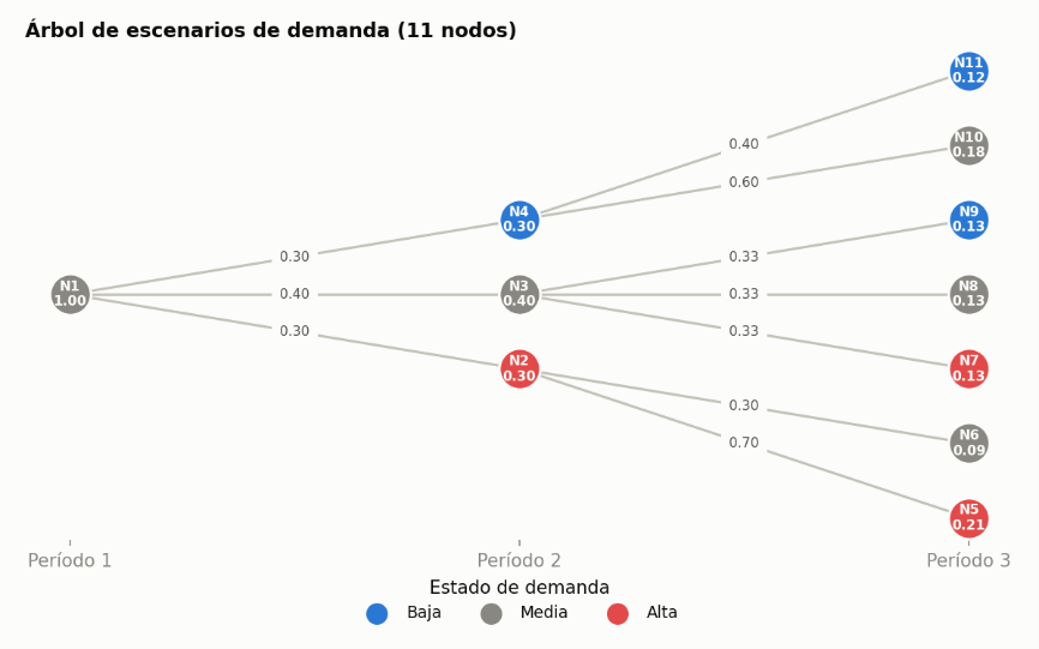
\includegraphics[width=0.75\textwidth]{./figuras/Grafo demanda.png}\par
  \vspace{0.6em}
  {\raggedright \small \textit{Nota.} Estructura compuesta por tres períodos y 11 nodos. Elaboración propia a partir de los datos proporcionados para el proyecto.\par}
\end{figure}

La Figura~\ref{fig:anexo_demanda_esperada} presenta la demanda esperada de cada combinación vino--etiqueta, ponderada por la probabilidad de los nodos terminales del árbol de escenarios.

\begin{figure}[H]
  \centering
  \caption{Demanda esperada por producto}
  \label{fig:anexo_demanda_esperada}
  \vspace{0.4em}
  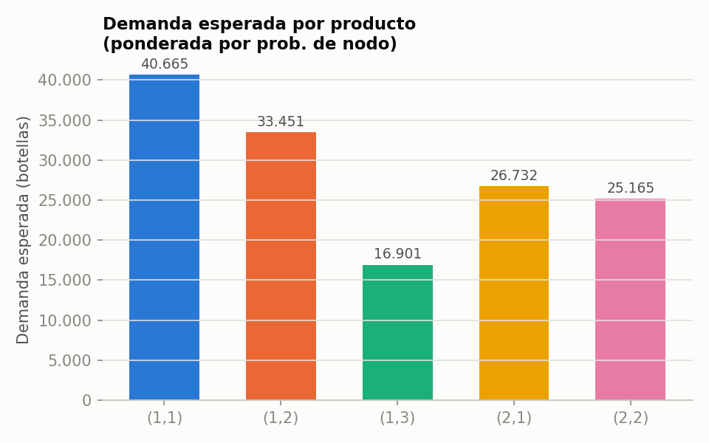
\includegraphics[width=0.75\textwidth]{./figuras/demanda esperada.png}\par
  \vspace{0.6em}
  {\raggedright \small \textit{Nota.} Valores expresados para cada combinación vino--etiqueta y ponderados por la probabilidad de los nodos terminales. Elaboración propia.\par}
\end{figure}

La Figura~\ref{fig:anexo_correlacion} presenta la matriz de correlación de la demanda entre los productos, calculada a partir de los 11 nodos del árbol de escenarios.

\begin{figure}[H]
  \centering
  \caption{Correlación de la demanda entre productos}
  \label{fig:anexo_correlacion}
  \vspace{0.4em}
  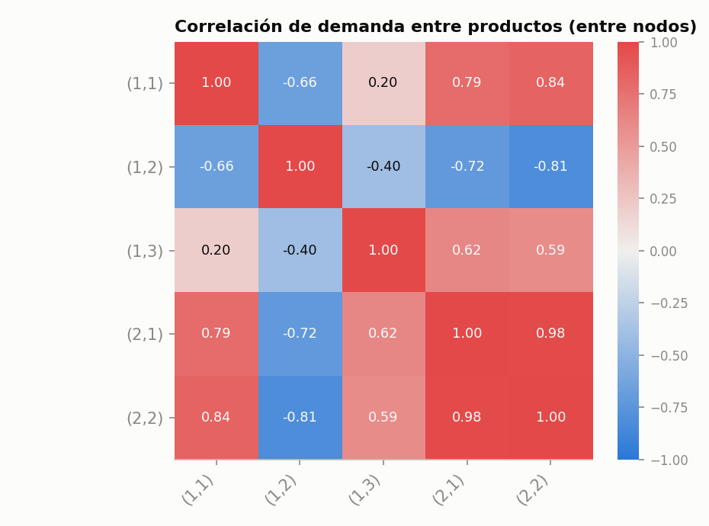
\includegraphics[width=0.75\textwidth]{./figuras/correlación demanda.png}\par
  \vspace{0.6em}
  {\raggedright \small \textit{Nota.} Matriz calculada a través de los 11 nodos del árbol de escenarios. Elaboración propia.\par}
\end{figure}

\newpage

% Anexo C (Tabla Comparativa)
\chapter{Tablas}
\label{anexo:tabla_comparativa}
\begin{table}[H]
  \centering
  \caption{Configuración del sistema de envasado}
  \label{tab:anexoA-configuracion}

  \begin{tabular*}{\textwidth}{@{\extracolsep{\fill}}>{\raggedright\arraybackslash}p{0.32\textwidth} c c >{\raggedright\arraybackslash}p{0.40\textwidth}}
    \toprule
    \textbf{Parámetro} & \textbf{Valor} & \textbf{Unidad} & \textbf{Comentario} \\
    \midrule
    Líneas de producción & 1 & línea & Realiza embotellado y etiquetado, acoplados o desacoplados \\
    Capacidad de la línea por período & 84 & horas & Tiempo disponible para producción y set-ups \\
    Períodos del horizonte & 3 & períodos & Coinciden con las etapas del árbol de escenarios \\
    Estanques intermedios disponibles & 20 & estanques & Número máximo utilizable en cada período \\
    Capacidad de cada estanque & 10.000 & litros & Un estanque alimenta la línea de embotellado \\
    Tamaño de botella (todos los vinos) & 0,75 & litros & $\approx$ 13.333 botellas por estanque \\
    Subutilización máxima de un estanque & 100\% & fracción & No se exige uso mínimo del estanque \\
    \bottomrule
  \end{tabular*}
\end{table}

\begin{table}[H]
  \centering
  \caption{Productos, etiquetas admisibles e inventarios iniciales}
  \label{tab:anexoA-productos}

  % Panel A
  \begin{tabular*}{\textwidth}{@{\extracolsep{\fill}}>{\raggedright\arraybackslash}p{0.20\textwidth} >{\raggedright\arraybackslash}p{0.35\textwidth} >{\raggedright\arraybackslash}p{0.38\textwidth}}
    \multicolumn{3}{@{}l}{\textbf{Panel A.} \textit{Productos y etiquetas admisibles}} \\[0.4em]
    \toprule
    \textbf{Vino} & \textbf{Etiquetas admisibles} & \textbf{Productos terminados (vino, etiqueta)} \\
    \midrule
    Vino 1 & Etiquetas 1, 2 y 3 & (1,1), (1,2), (1,3) \\
    Vino 2 & Etiquetas 1 y 2    & (2,1), (2,2) \\
    \bottomrule
  \end{tabular*}

  \vspace{1.2em}

  % Panel B
  \begin{tabular*}{\textwidth}{@{\extracolsep{\fill}}>{\raggedright\arraybackslash}p{0.55\textwidth} c >{\raggedright\arraybackslash}p{0.30\textwidth}}
    \multicolumn{3}{@{}l}{\textbf{Panel B.} \textit{Inventario inicial}} \\[0.4em]
    \toprule
    \textbf{Inventario inicial} & \textbf{Valor} & \textbf{Unidad} \\
    \midrule
    Botellas llenas sin etiquetar (ambos vinos)    & 0 & botellas \\
    Productos terminados (todas las combinaciones) & 0 & botellas \\
    Pedidos atrasados (\textit{backlog}) iniciales   & 0 & botellas \\
    \bottomrule
  \end{tabular*}

  \vspace{0.6em}
  \raggedright \small \textit{Nota.} La demanda del período 1 (nodo 1) se satisface con actividades de embotellado y etiquetado predefinidas, iguales a la demanda de ese nodo.
\end{table}

\begin{table}[H]
  \centering
  \caption{Tiempos y costos de operación}
  \label{tab:anexoA-tiempos-costos}

  % Panel A
  \begin{tabular*}{\textwidth}{@{\extracolsep{\fill}}>{\raggedright\arraybackslash}p{0.52\textwidth} c r}
    \multicolumn{3}{@{}l}{\textbf{Panel A.} \textit{Tiempos y costos de preparación (set-ups)}} \\[0.4em]
    \toprule
    \textbf{Concepto} & \textbf{Tiempo (h)} & \textbf{Costo (\$)} \\
    \midrule
    Set-up de embotellado & 1,5 & 1.500 \\
    Set-up conjunto de embotellado y etiquetado & 1,5 & 1.500 \\
    Set-up de etiquetado & 0,5 & 500 \\
    \bottomrule
  \end{tabular*}

  \vspace{1.2em}

  % Panel B
  \begin{tabular*}{\textwidth}{@{\extracolsep{\fill}}>{\raggedright\arraybackslash}p{0.52\textwidth} c r}
    \multicolumn{3}{@{}l}{\textbf{Panel B.} \textit{Tiempos unitarios de proceso}} \\[0.4em]
    \toprule
    \textbf{Proceso} & \textbf{Valor (h/botella)} & \textbf{Unidad} \\
    \midrule
    Llenado (solo embotellar) & 0,00014 & h/botella \\
    Etiquetado (solo etiquetar) & 0,00028 & h/botella \\
    Llenado y etiquetado acoplados & 0,00028 & h/botella \\
    \bottomrule
  \end{tabular*}

  \vspace{1.2em}

  % Panel C
  \begin{tabular*}{\textwidth}{@{\extracolsep{\fill}}>{\raggedright\arraybackslash}p{0.52\textwidth} c r}
    \multicolumn{3}{@{}l}{\textbf{Panel C.} \textit{Costos de inventario y servicio}} \\[0.4em]
    \toprule
    \textbf{Costo de inventario y servicio} & \textbf{Valor} & \textbf{Unidad} \\
    \midrule
    Mantener una botella llena sin etiquetar & 10 & \$/botella$\cdot$período \\
    Mantener una botella de producto terminado & 15 & \$/botella$\cdot$período \\
    Pedido atrasado (\textit{backorder}) & 15.000 & \$/botella$\cdot$período \\
    \bottomrule
  \end{tabular*}
\end{table}

\begin{table}[H]
  \centering
  \caption{Árbol de escenarios de demanda}
  \label{tab:anexoA-arbol-escenarios}

  \begin{tabular*}{\textwidth}{@{\extracolsep{\fill}}cccccc}
    \toprule
    \textbf{Nodo} & \textbf{Período} & \textbf{Estado} & \textbf{Nodo antecesor} & \textbf{Prob. condicional} & \textbf{Prob. del nodo} \\
    \midrule
    1  & 1 & Media & — & 1,000 & 1,000 \\
    2  & 2 & Alta  & 1 & 0,300 & 0,300 \\
    3  & 2 & Media & 1 & 0,400 & 0,400 \\
    4  & 2 & Baja  & 1 & 0,300 & 0,300 \\
    5  & 3 & Alta  & 2 & 0,700 & 0,210 \\
    6  & 3 & Media & 2 & 0,300 & 0,090 \\
    7  & 3 & Alta  & 3 & 0,333 & 0,133 \\
    8  & 3 & Media & 3 & 0,333 & 0,133 \\
    9  & 3 & Baja  & 3 & 0,333 & 0,133 \\
    10 & 3 & Media & 4 & 0,600 & 0,180 \\
    11 & 3 & Baja  & 4 & 0,400 & 0,120 \\
    \bottomrule
  \end{tabular*}

  \vspace{0.6em}
  \raggedright \small \textit{Nota.} Árbol de 3 períodos y 11 nodos. La probabilidad de cada nodo es el producto de las probabilidades condicionales desde la raíz; las probabilidades de los nodos terminales suman 1.
\end{table}

\begin{table}[H]
  \centering
  \caption{Demanda por producto y nodo}
  \label{tab:anexoA-demanda}

  \small
  \setlength{\tabcolsep}{3pt} % Reduce el espacio horizontal entre columnas
  \begin{tabular*}{\textwidth}{@{\extracolsep{\fill}} l *{11}{r} }
    \toprule
    \textbf{Producto} & \textbf{N1} & \textbf{N2} & \textbf{N3} & \textbf{N4} & \textbf{N5} & \textbf{N6} & \textbf{N7} & \textbf{N8} & \textbf{N9} & \textbf{N10} & \textbf{N11} \\
    \midrule
    (1,1) & 23.525 & 53.218 & 34.328 & 18.118 & 81.856 & 45.302 & 50.426 & 31.482 & 12.538 & 30.856 & 10.426 \\
    (1,2) & 24.328 & 15.184 & 28.525 & 45.832 & 24.546 & 31.371 & 23.569 & 40.767 & 57.965 & 20.546 & 45.569 \\
    (1,3) & 20.368 & 38.150 & 21.080 & 6.762  & 4.920  & 25.765 & 35.043 & 25.646 & 16.248 & 10.920 & 11.043 \\
    (2,1) & 21.080 & 39.387 & 30.368 & 12.646 & 34.115 & 22.773 & 37.045 & 27.831 & 18.616 & 24.115 & 17.045 \\
    (2,2) & 22.991 & 38.048 & 27.991 & 14.949 & 33.440 & 22.824 & 35.085 & 25.147 & 15.209 & 23.440 & 15.085 \\
    \bottomrule
  \end{tabular*}

  \vspace{0.6em}
  \raggedright \small \textit{Nota.} Demanda expresada en botellas. La demanda de un nodo debe atenderse en ese nodo; lo no atendido queda como pedido atrasado. Las demandas de los productos del Vino 1 presentan correlaciones negativas entre sí; las del Vino 2, positivas (ver Sección 4.4).
\end{table}

\begin{table}[H]
  \centering
  \caption{Matriz comparativa de metodologías de IO para el proceso de envasado y postergación}
  \label{tab:comparativa_metodologias}

  \small
  \setlength{\tabcolsep}{3pt} % Controla el espacio entre columnas para evitar desbordes
  \begin{tabular*}{\textwidth}{@{\extracolsep{\fill}}
    >{\raggedright\arraybackslash}p{0.15\textwidth} 
    >{\raggedright\arraybackslash}p{0.18\textwidth} 
    >{\raggedright\arraybackslash}p{0.18\textwidth} 
    >{\raggedright\arraybackslash}p{0.18\textwidth} 
    >{\raggedright\arraybackslash}p{0.16\textwidth}}
    \toprule
    \textbf{Método} & \textbf{Manejo de Incertidumbre} & \textbf{Manejo de \textit{Set-ups} y Tiempos} & \textbf{Ventaja Principal} & \textbf{Desventaja Principal} \\
    \midrule

    \textbf{Optimización Estocástica (2 Etapas)} & Árboles discretos / probabilidades condicionales \cite{gupta2000two}. & \textit{Set-ups} de embotellado en Etapa 1; WIP y penalizaciones en Etapa 2. & Cuantifica el valor del \textit{postponement}, VSS y \textit{risk pooling} ($r = 0{,}66$). & Explosión combinatoria de escenarios si aumenta el árbol. \\
    \addlinespace[0.5em]

    \textbf{MILP Determinista (Valor Esperado)} & Ignora aleatoriedad; usa demandas promediadas \cite{gunther2014block}. & Excelente para \textit{set-ups} dependientes de la secuencia y filtros \cite{lillo2025optimal}. & Alta velocidad de cómputo en \textit{solvers} como Gurobi. & Inflexible; ignora variabilidad y subestima pedidos atrasados. \\
    \addlinespace[0.5em]

    \textbf{Programación Robusta (ARO)} & Conjuntos poliédricos; optimiza para el peor escenario \cite{hu2020hybrid}. & Introduce \textit{time gaps} entre corridas de producción \cite{lappas2016multi}. & Inmune a variaciones extremas; no requiere de distribuciones previas. & ``Precio de la Robustez'' elevado; inventario WIP conservador e innecesario. \\
    \addlinespace[0.5em]

    \textbf{Simulación Monte Carlo / DES} & Muestreo estocástico de trayectorias \cite{review2024simula}. & Representación detallada de fallas y tiempos no lineales \cite{jeon2016survey}. & Excelente para pruebas de estrés y validación operacional. & Herramienta puramente descriptiva, no prescriptiva; no genera planes óptimos. \\
    \bottomrule
  \end{tabular*}
\end{table}

\begin{table}[H]
  \centering
  \caption{Dimensiones consideradas en los escenarios experimentales}
  \label{tab:escenarios_metodologicos}

  \small
  \setlength{\tabcolsep}{4pt}
  \begin{tabular*}{\textwidth}{@{\extracolsep{\fill}}
    >{\raggedright\arraybackslash}p{0.25\textwidth} 
    >{\raggedright\arraybackslash}p{0.30\textwidth} 
    >{\raggedright\arraybackslash}p{0.40\textwidth}}
    \toprule
    \textbf{Dimensión} & \textbf{Niveles} & \textbf{Interpretación} \\
    \midrule
    Variabilidad de demanda
    & $10\%$, $30\%$, $50\%$
    & Intensidad de la incertidumbre respecto de la demanda media. \\
    \addlinespace[0.4em]

    Capacidad de línea
    & 21, 42, 63 y 84 h/período
    & Grado de holgura disponible para absorber producción, recurso y \textit{set-ups}. \\
    \addlinespace[0.4em]

    Nivel de postergación
    & $PL \in \{0,2,3,4,5\}$
    & Número máximo de etiquetas para las cuales se permite mantener flexibilidad mediante diferenciación tardía. \\
    \addlinespace[0.4em]

    Correlación de demanda
    & Positiva / negativa
    & Grado en que la demanda de productos se mueve conjuntamente o presenta compensaciones entre etiquetas. \\
    \bottomrule
  \end{tabular*}
\end{table}

\newpage

% Anexo D (Restricciones)
\chapter{Restricciones del modelo}
\label{anexo:restricciones}
Esta sección presenta, a modo de referencia autocontenida, la formulación
matemática preliminar de las principales restricciones del modelo descritas
conceptualmente en el cuerpo del informe. Las expresiones corresponden a una
primera propuesta de modelación y podrán ser ajustadas durante las etapas
posteriores de implementación, verificación y validación.

\subsection*{D.1. Balance del inventario intermedio}

El inventario de botellas sin etiquetar debe conservar el flujo físico del
vino. Dado que el embotellado tiene un tiempo de disponibilidad de una etapa,
se plantea:

\begin{equation}
    s^{b}_{in}
    =
    s^{b}_{i,a(n)}
    +
    w^{b}_{i,a(n)}
    -
    \sum_{j\in J_i} w^{l}_{ijn},
    \qquad \forall i,n.
    \label{eq:anexoD-balance-intermedio}
\end{equation}

La producción sin etiquetar realizada en el nodo antecesor se encuentra
disponible en el nodo $n$, mientras que el etiquetado realizado en $n$ puede
consumir dicho inventario después de observar la demanda correspondiente al
nodo.

Adicionalmente, la cantidad etiquetada no puede superar el inventario de
botellas sin etiquetar efectivamente disponible:

\begin{equation}
    \sum_{j\in J_i} w^{l}_{ijn}
    \leq
    s^{b}_{i,a(n)}
    +
    w^{b}_{i,a(n)},
    \qquad \forall i,n.
    \label{eq:anexoD-disponibilidad-intermedia}
\end{equation}


\subsection*{D.2. Balance de producto terminado y pedidos atrasados}

Para cada combinación vino--etiqueta $(i,j)$, el inventario de producto
terminado y los pedidos atrasados deben satisfacer:

\begin{equation}
    s^{bl}_{ijn}
    -
    b^{bl}_{ijn}
    =
    s^{bl}_{ij,a(n)}
    -
    b^{bl}_{ij,a(n)}
    +
    w^{bl}_{ij,a(n)}
    +
    w^{l}_{ijn}
    -
    D_{ijn},
    \qquad \forall i,j,n.
    \label{eq:anexoD-balance-terminado}
\end{equation}

La producción acoplada disponible en el nodo $n$ corresponde a una decisión
realizada en su nodo antecesor, mientras que el etiquetado de inventario
intermedio puede reaccionar a la demanda observada en $n$. De esta forma, la
postergación permite desplazar parte de la diferenciación hacia un momento en
que se dispone de mayor información.


\subsection*{D.3. Capacidad de la línea}

La única línea disponible comparte su capacidad entre las operaciones de
embotellado, embotellado y etiquetado acoplados, etiquetado posterior y sus
respectivos \textit{set-ups}. Para cada nodo:

\begin{equation}
\begin{aligned}
    &0{,}00014\sum_i w^{b}_{in}
    +
    0{,}00028\sum_i\sum_{j\in J_i} w^{bl}_{ijn}
    +
    0{,}00028\sum_i\sum_{j\in J_i} w^{l}_{ijn}
    \\
    &\quad+
    1{,}5\sum_i z^{b}_{in}
    +
    1{,}5\sum_i\sum_{j\in J_i} z^{bl}_{ijn}
    +
    0{,}5\sum_i\sum_{j\in J_i} z^{l}_{ijn}
    \leq C,
    \qquad \forall n.
\end{aligned}
\label{eq:anexoD-capacidad}
\end{equation}

donde la capacidad disponible depende del escenario experimental considerado:

\begin{equation}
    C \in \{21,42,63,84\}.
    \label{eq:anexoD-niveles-capacidad}
\end{equation}

Esta restricción refleja que la postergación no constituye una fuente de
flexibilidad gratuita. Una botella que sigue la ruta desacoplada consume
capacidad durante el embotellado y vuelve a utilizarla posteriormente durante
el etiquetado. Por lo tanto, el beneficio de esperar nueva información debe
compensar el uso adicional de capacidad productiva.


\subsection*{D.4. Activación de \textit{set-ups}}

Las cantidades procesadas deben encontrarse asociadas a las variables binarias
que representan la activación de los \textit{set-ups} correspondientes. Se
plantean las siguientes relaciones:

\begin{equation}
    w^{b}_{in}
    \leq
    M^{b}(C)z^{b}_{in},
    \qquad \forall i,n,
    \label{eq:anexoD-setup-embotellado}
\end{equation}

\begin{equation}
    w^{bl}_{ijn}
    \leq
    M^{bl}(C)z^{bl}_{ijn},
    \qquad \forall i,j,n,
    \label{eq:anexoD-setup-acoplado}
\end{equation}

\begin{equation}
    w^{l}_{ijn}
    \leq
    M^{l}(C)z^{l}_{ijn},
    \qquad \forall i,j,n.
    \label{eq:anexoD-setup-etiquetado}
\end{equation}

Para evitar utilizar constantes $M$ excesivamente grandes, sus cotas se
derivan directamente de la capacidad disponible:

\begin{equation}
    M^{b}(C)
    =
    \max
    \left\{
        \frac{C-1{,}5}{0{,}00014},
        0
    \right\},
    \label{eq:anexoD-bigM-embotellado}
\end{equation}

\begin{equation}
    M^{bl}(C)
    =
    \max
    \left\{
        \frac{C-1{,}5}{0{,}00028},
        0
    \right\},
    \label{eq:anexoD-bigM-acoplado}
\end{equation}

\begin{equation}
    M^{l}(C)
    =
    \max
    \left\{
        \frac{C-0{,}5}{0{,}00028},
        0
    \right\}.
    \label{eq:anexoD-bigM-etiquetado}
\end{equation}

Estas cotas dependen del escenario de capacidad y evitan utilizar valores
arbitrariamente grandes de $M$ que puedan deteriorar innecesariamente la
relajación lineal del modelo.


\subsection*{D.5. Compatibilidad entre vinos y etiquetas}

El inventario de botellas sin etiquetar conserva flexibilidad únicamente entre
productos asociados al mismo vino base. Para la instancia analizada:

\begin{equation}
    J_1 = \{1,2,3\},
    \qquad
    J_2 = \{1,2\}.
    \label{eq:anexoD-compatibilidad}
\end{equation}

Por lo tanto, una botella correspondiente al Vino 1 puede transformarse en los
productos $(1,1)$, $(1,2)$ o $(1,3)$, mientras que una botella correspondiente
al Vino 2 puede asignarse únicamente a $(2,1)$ o $(2,2)$. En consecuencia, el
efecto de \textit{risk pooling} generado por la postergación ocurre entre
etiquetas que comparten el mismo vino base y no entre vinos diferentes.


\subsection*{D.6. Disponibilidad de estanques}

Los 20 estanques de 10.000 litros corresponden al vino preparado para alimentar
el proceso de embotellado y no representan capacidad de almacenamiento de
botellas sin etiquetar.

Sea $y_{in}$ el número entero de estanques preparados para el vino $i$ en el
nodo $n$, y $u_{in}$ su subutilización. El número de estanques utilizados debe
satisfacer:

\begin{equation}
    \sum_i y_{in}
    \leq
    20,
    \qquad \forall n.
    \label{eq:anexoD-numero-estanques}
\end{equation}

El volumen preparado se relaciona con la cantidad de botellas procesadas
mediante:

\begin{equation}
    10.000
    \left(
        y_{in}-u_{in}
    \right)
    =
    0{,}75
    \left(
        w^{b}_{in}
        +
        \sum_{j\in J_i} w^{bl}_{ijn}
    \right),
    \qquad \forall i,n.
    \label{eq:anexoD-balance-estanques}
\end{equation}

Dado que la subutilización máxima admisible de un estanque es del 100\%, no se
exige una utilización mínima de cada estanque. Sin embargo, el número total de
estanques continúa restringiendo físicamente el volumen de vino que puede
encontrarse preparado simultáneamente para alimentar la línea.


\subsection*{D.7. Condiciones iniciales y frontera temporal}

Los inventarios iniciales de botellas sin etiquetar, productos terminados y
pedidos atrasados son iguales a cero. La demanda correspondiente al nodo raíz
se satisface mediante actividades predefinidas de embotellado y etiquetado
equivalentes a la demanda de dicho nodo. Esta condición permite iniciar el
árbol desde un estado conocido y concentrar las decisiones de optimización en
la respuesta a la incertidumbre futura.

Asimismo, dado que el embotellado requiere una etapa para encontrarse
disponible, las decisiones adoptadas al final del horizonte no deben generar
artificialmente valor asociado a producto cuya disponibilidad se produzca
fuera de los tres períodos considerados.

El tratamiento de las variables terminales deberá revisarse en la formulación
definitiva, evitando incentivar producción cuya disponibilidad ocurra después
del tercer período, salvo que se incorpore explícitamente una condición de
valor residual.

% Agregar más anexos de ser necesario
%\chapter*{Anexo N°2: Datos adicionales}
%\addcontentsline{toc}{chapter}{Anexo N°2: Datos adicionales}
%\input{./Secciones/anexo2.tex}

\end{document}